
The first tutorial shows how to create a dike with multiple layers and multiple piezometric levels. Note that this tutorial is meant to show the possibilities of KratosGeoMechanics in GiD, rather than creating a realistic dike. 
\section{Geometry}	
\begin{enumerate}
	
	
	\item In GiD, press the icon  \includegraphics{CreateLine.png} and draw the outlines of your geometry according to Table \ref{tab:tut1_outline}. Make sure to press "Join" in the Create point procedure when connecting the last line to the first point.

%		\begin{table}[h!]
%		\centering
%		\caption{Outline geometry tutorial 1}
%		\label{tab:tut1_outline}
%		\begin{tabular}{llll}
%			Point ID & x-coordinate & y-coordinate & Escape \\
%			1        & -50, -15     & 50, -15      & False	\\
%			2        & 50           & -15          & False  \\
%			3        & 40           & 0            & False  \\
%			4        & 10           & 0            & False  \\
%			5        & 0            & 5            & False  \\
%			6        & -5           & 5            & False  \\
%			7        & -15          & 0            & False  \\
%			8        & -50          & 0            & False  \\
%			1        & -50          & -15          & True
%		\end{tabular}
%	\end{table}

	\begin{table}[h!]
		\centering
		\caption{Outline geometry tutorial 1}
		\label{tab:tut1_outline}
		\begin{tabular}{lll}
			Line ID  & Point 1 (x,y)& Point 2 (x,y) \\
			1        & -50, -15     & 50, -15      \\
			2        & 50, -15      & 50, 0        \\
			3        & 50, 0        & 10, 0        \\
			4        & 10, 0        & 0, 5         \\
			5        & 0, 5         & -5, 5        \\
			6        & -5, 5        & -15, 0       \\
			7        & -15, 0       & -50, 0       \\
			8        & -50, 0       & -50, -15     \\
		\end{tabular}
	\end{table}


	\item Now create lines to set the outlines of the soil layers. According to Table \ref{tab:tut1_outline_sl}.
%	\begin{table}[h!]
%		\centering
%		\caption{Outline soil layer tutorial 1}
%		\label{tab:tut1_outline_sl}
%		\begin{tabular}{llll}
%			Point ID & x-coordinate & y-coordinate & Escape \\
%			9        & -50, -10     & -10          & False	\\
%			10       & 50           & -10          & True  \\
%			7        & -15          & 0            & False  \\
%			4        & 10           & 0            & True  \\
%		\end{tabular}
%	\end{table}


		\begin{table}[h!]
		\centering
		\caption{Outline soil layer tutorial 1}
		\label{tab:tut1_outline_sl}
		\begin{tabular}{lll}
			Line ID  & Point 1 (x,y)& Point 2 (x,y) \\
			9        & (-50, -10)     & (50, -10)      \\
			10       & (-15, 0)       & (10, 0 )         \\
		\end{tabular}
	\end{table}


	\item Create vertical lines at the location of the turning points of the phreatic level which will be created in a further step, according to Table \ref{tab:tut1_verticals_water}. 
%	\begin{table}[h!]
%		\centering
%		\caption{Verticals turning points phreatic line tutorial 1}
%		\label{tab:tut1_verticals_water}
%		\begin{tabular}{llll}
%			Point ID & x-coordinate  & y-coordinate & Escape \\
%			11       & -7.5          & 5            & False	\\
%			12       & -7.5          & -15          & True  \\
%			4        & -15           & 0            & False \\
%			13       & 10            & 0             & True  \\
%		\end{tabular}
%	\end{table}

	\begin{table}[h!]
		\centering
		\caption{Verticals turning points phreatic line tutorial 1}
		\label{tab:tut1_verticals_water}
		\begin{tabular}{lll}
			Line ID  & Point 1 (x,y)& Point 2 (x,y) \\
			11       & (-7.5, 5)       & (-7.5, -15) \\
			12       & (-15, 0)        & (10, 0) \\
		\end{tabular}
	\end{table}




	\item Create all the intersections between the lines by clicking on the 
\includegraphics{divideLineAtIntersectLine.png} button and selecting everything. The outlines should look as displayed in Figure \ref{fig:tut1_all_outline}. Further references to line ID's are done using the line ID's as shown in the figure.
	
	\begin{figure}[h!]		
		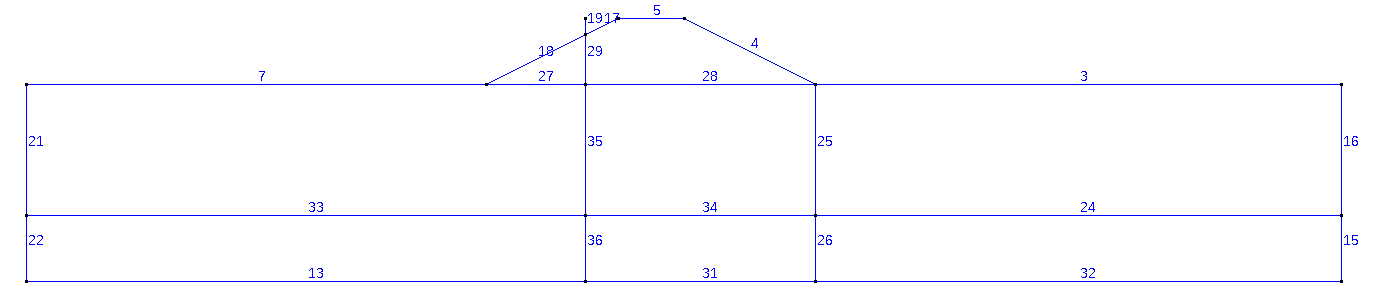
\includegraphics[width=0.9\textwidth]{outlinesTutorial1.png}
		\caption{All outlines tutorial 1}
		\label{fig:tut1_all_outline}
	\end{figure}

	\item Create surfaces by clicking on the 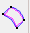
\includegraphics{createNurbsSurface.png} button and selecting the lines as displayed in Table \ref{tab:tut1_surfaces}. 
	
	 	\begin{table}[h!]
	 	\centering
	 	\caption{Surfaces tutorial 1}
	 	\label{tab:tut1_surfaces}
	 	\begin{tabular}{ll}
	 		Surface ID  & line ID's \\
	 		1       & (7, 27, 35, 33, 21) \\
	 		2       & (28, 25, 34, 35) \\
	 		3       & (3, 16, 24, 25) \\
	 		4       & (33, 36, 13, 22) \\
	 		5       & (34, 26, 31, 36) \\
	 		6       & (24, 15, 32, 26) \\
	 		7       & (18, 29, 27) \\
	 		8       & (17, 5, 4, 28, 29) \\
	 	\end{tabular}
	 \end{table}
 
 	\item Delete line (19) and the attached point by clicking on the 
\includegraphics{deleteButton.png} and the 
\includegraphics{deleteAllButton.png} in the Geometry toolbar. The geometry should look like as displayed in Figure \ref{fig:tut1_geometry}. Further references to surface ID's are made to the ID's as shown in the figure. 
 
 	\begin{figure}[h!]		
 		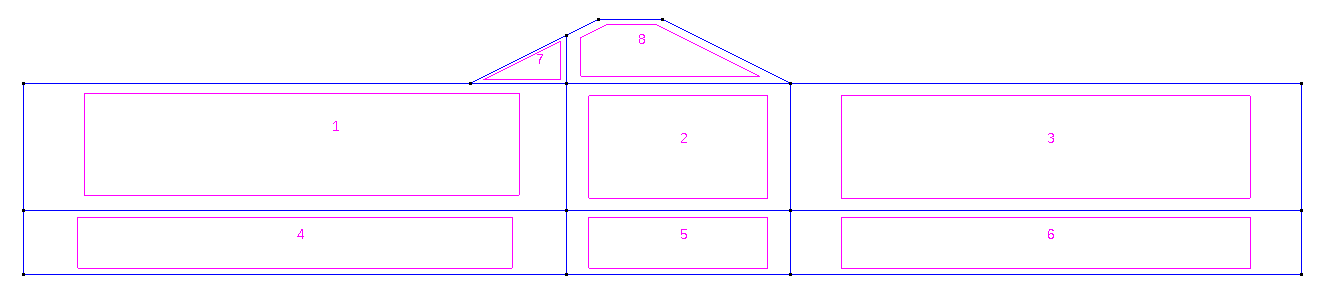
\includegraphics[width=0.9\textwidth]{geometryTut1.png}
 		\caption{Geometry tutorial 1}
 		\label{fig:tut1_geometry}
 	\end{figure}
 
 
\end{enumerate}
\section{Boundary conditions}

\begin{enumerate}[resume]


	\item The next step is setting the boundary conditions. In this tutorial, the side boundaries can move freely in vertical direction; the bottom boundary is fixed. In the top menu bar, select \textit{GeoMechanicsApplication->Dirichlet Constraints}. The window as shown in Figure \ref{fig:tut1_dirichlet_constraints_window} should appear. 
	\begin{figure}[h!]		
		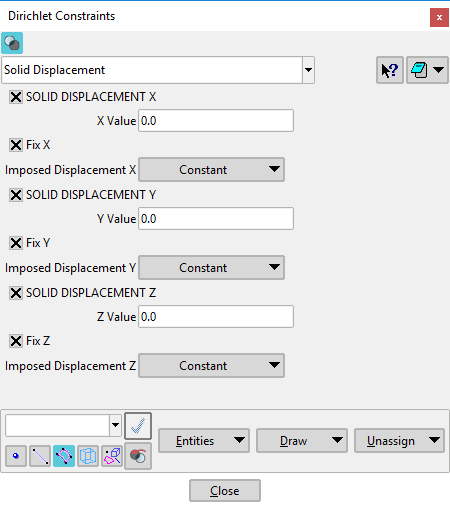
\includegraphics[width=0.5\textwidth]{dirichletConstraintsWindow.png}
		\caption{Dirichlet constraints window}
		\label{fig:tut1_dirichlet_constraints_window}
	\end{figure}

	\item For the side boundaries, deselect "\textit{SOLID DISPLACEMENT Y}". Now in the bottom left corner of the Dirichlet Constaints window, fill in "side boundary". In this same window click on the line button 
\includegraphics{assignToLine.png}. And click on the create new group button, 
\includegraphics{createNewGroup}. Now select the lines (21, 22, 15, 16) in the geometry and press "ESC".
	
	\item For the bottom boundary, in the Dirichlet Constaints window, select all the \textit{SOLID DISPLACEMENT} buttons and keep the values at 0. Name this boundary "bottom boundary", and assign this boundary condition to the lines (13, 31 ,32).
\end{enumerate}
\section{Materials}
\begin{enumerate}[resume]	
	\item Now the materials have to be assigned to the surfaces. In this tutorial, 3 materials will be created. In the top menu bar, select \textit{GeoMechanicsApplication->Elements}. A new window should appear.
	
	\item In the elements window which appeared, from the top drop-down menu, select "soil-drained". And fill in the values as shown in Figure \ref{fig:tut1_clay_mat}. For the parameter, "UDSM Name", fill in the address of the "MohrCoulomb.dll", including extension. For the description of the Mohr Coulomb parameters, see @@@. Assign the material to the surfaces (1, 2, 3).
	
	\begin{figure}[h!]		
		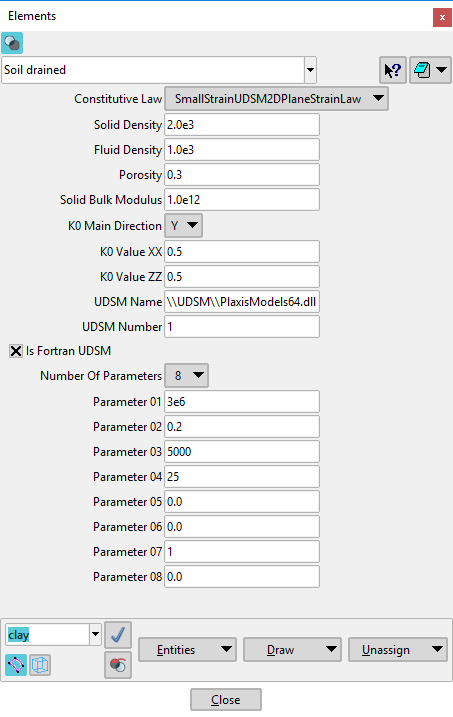
\includegraphics[width=0.5\textwidth]{clayMaterialWindowTut1.png}
		\caption{Clay parameters tutorial 1}
		\label{fig:tut1_clay_mat}
	\end{figure}
	
	\item For the second material, select "soil-drained" and fill in the parameters as shown in Figure \ref{fig:tut1_sand_mat}. Again for the "UDSM Name" fill in the address if the "MohrCoulomb.dll", including extension. Assign the material to the surfaces (4, 5, 6)
	
	\begin{figure}[h!]		
		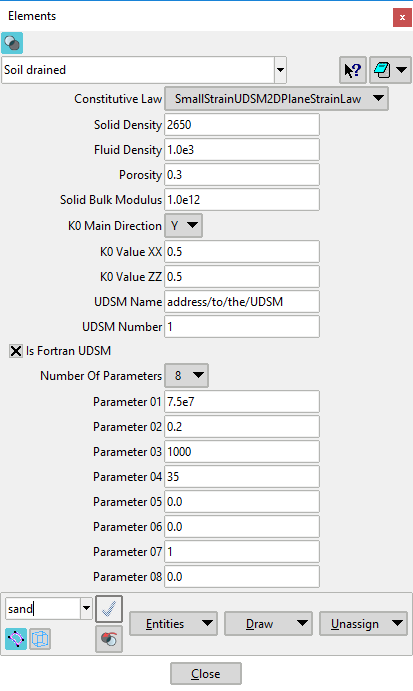
\includegraphics[width=0.5\textwidth]{sandMaterialWindowTut1.png}
		\caption{Sand parameters tutorial 1}
		\label{fig:tut1_sand_mat}
	\end{figure}

	\item For the last material, again select "soil-drained" and fill in the parameters as shown in Figure \ref{fig:tut1_dike_mat}, again referring to "MohrCoulomb.dll" for "UDSM Name". Assign the material to surfaces (7, 8).
	
	\begin{figure}[h!]		
		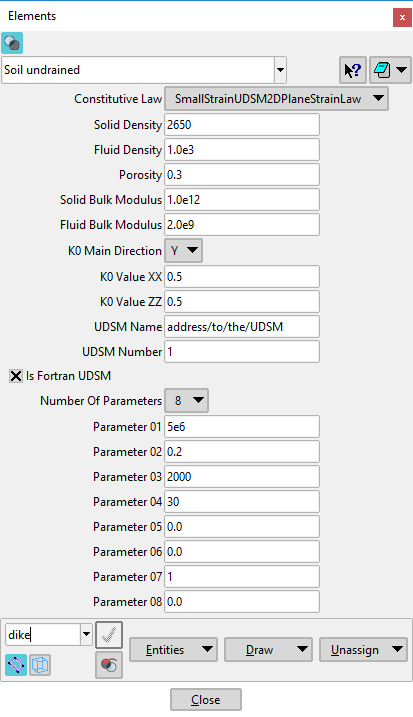
\includegraphics[width=0.5\textwidth]{dikeMaterialWindowTut1.png}
		\caption{Dike parameters tutorial 1}
		\label{fig:tut1_dike_mat}
	\end{figure}
\end{enumerate}

\section{Water}
\begin{enumerate}[resume]
	\item The first water level to be added is the river water level. Click on \textit{GeoMechanicsApplication -> Dirichlet Constraints}. In the Dirichlet Constraints window, select Fluid Pressure from the top drop-down menu. Fill in the parameters as shown in Figure \ref{fig:tut1_river_level}. Assign this fluid pressure to line 7.
	
	\begin{figure}[h!]		
		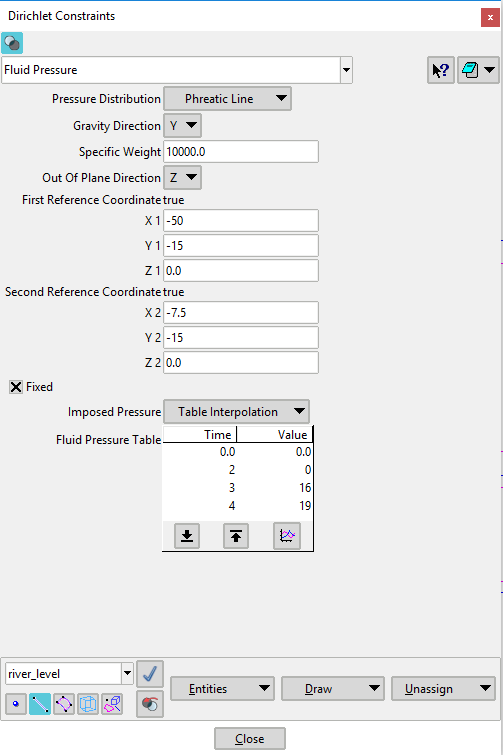
\includegraphics[width=0.5\textwidth]{riverLevelTut1.png}
		\caption{River water level tutorial 1}
		\label{fig:tut1_river_level}
	\end{figure}
	
	\item Now rename the previous Fluid pressure condition to "\verb|river_level_surface|". And assign the condition to surface 7
	
	\item The water pressure due to the river water level is now set, however since the water level lies above the surface, it is required to explicitly define the normal load due to the water. Click on \textit{GeoMechanicsApplication -> Loads}. From the top drop-down menu in de Loads window, select \textit{Normal Load}. Fill in the values as shown in Figure \ref{fig:tut1_river_load}. Assign the condition to the lines 17 and 18. 
		
	\begin{figure}[h!]		
		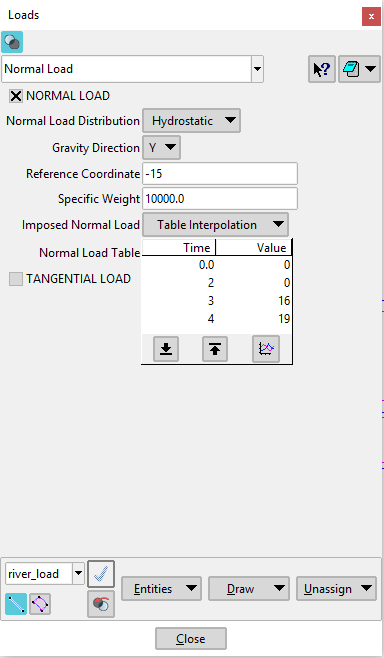
\includegraphics[width=0.5\textwidth]{riverLoadTut1.png}
		\caption{River load tutorial 1}
		\label{fig:tut1_river_load}
	\end{figure}

	\item The water level in the dike is an inclined phreatic line. Click on \textit{GeoMechanicsApplication -> Dirichlet Constraints}. Select \textit{Fluid Pressure} from the top drop-down menu in the Dirichlet Constraints table and fill in the values as shown in Figure \ref{fig:tut1_dike_level}. Assign the condition to surface 8. 
	
	\begin{figure}[h!]		
		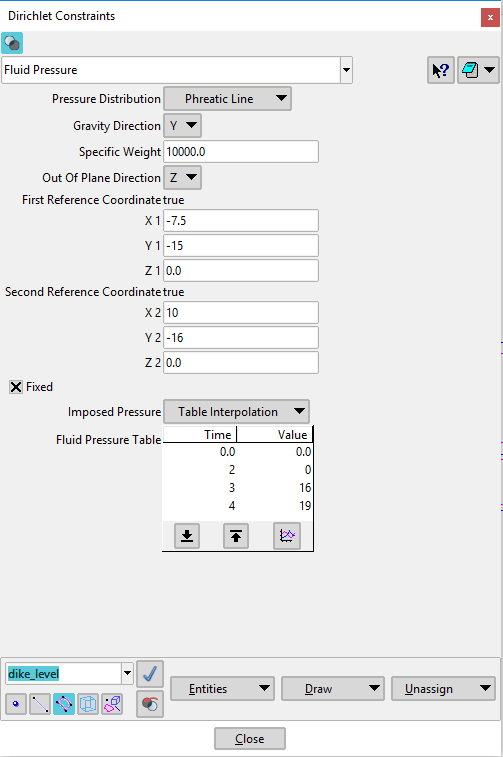
\includegraphics[width=0.5\textwidth]{dikeLevelTut1.png}
		\caption{Dike water level tutorial 1}
		\label{fig:tut1_dike_level}
	\end{figure}
	
	\item For the last part of the phreatic level, select \textit{fluid pressure}, choose \textit{Hydrostatic} pressure distribution. Set the reference coordinate on -15. In the Fluid pressure table fill in 0 on time 0 and 2; fill in 15 at time 3 and 4. Name the condition \verb|"polder level"| and assign the condition to line 3.
	
	\item Now for the water level in the aquifer, select \textit{fluid pressure}, choose \textit{Hydrostatic} pressure distribution. Set the reference coordinate on -15. In the Fluid pressure table fill in 0 on time 0 and 2; fill in 18 at time 3 and 4. Name the condition \verb|"aquifer_level"| and assign the condition to surface  4, 5 and 6.
	
	\item Lastly, select \textit{Interpolate line} pressure distribution, set \textit{Imposed Pressure} on \textit{Table Interpolation} and assign the condition to surface 1, 2 and 3.  
	
\end{enumerate}
\section{Loads}
\begin{enumerate}[resume]
	\item In this tutorial, the only loads will be applied are water loads and the own weight of the soils. The water loads are already applied in the previous section. To apply the soil weight, click on \textit{GeoMechanicsApplication -> Loads} and select  \textit{Body Acceleration} from the drop-down menu.
	
	\item In the Loads window, for \textit{Imposed Body Acceleration Y} select table interpolation. Fill in 0 for time 0; and fill in -9.81 for time 1 and 4. Name this load \verb|"body_surface"| and assign the condition to the surfaces: 1, 2, 3, 4, 5, 6. 
	
	\item For the self weight of the dike, in the Loads window, for \textit{Imposed Body Acceleration Y} select table interpolation. Fill in 0 for time 0 and 1; and fill in -9.81 for time 2 and 4. Name this load \verb|"body_dike"| and assign the condition to the surfaces: 7, 8.
		
\end{enumerate}

\section{Meshing}
\begin{enumerate}[resume]
	\item On the top menu bar, click on \textit{Mesh -> Unstructured -> Assign sizes on surfaces}. Fill in 1.0 in the dialog window which pops up. And assign this size on the surfaces 7 and 8.
	
	\item Now fill in 3.0 in the dialog window and assign this size to the surfaces: 1, 2, 3, 4, 5, 6. 
	
	\item On the top menu bar, click on \textit{Mesh -> Quadratic type -> Quadratic}. Such that quadratic elements are generated.
	\item On the top menu bar, click on \textit{Mesh -> Generate mesh...}. A Mesh generation window pops up where the element size of the mesh can be filled in. However, since the mesh size of all the surfaces is already defined in previous steps, the number which is filled in into the mesh generation window does not matter.  
\end{enumerate}


\section{Project Parameters}
\begin{enumerate}[resume]
	\item Before the model can be calculated, the project parameters should be filled in correctly. Click on \textit{GeoMechanicsApplication -> Project Parameters}. The problem data Window should appear.
	
	\item In the \textit{Problem data} window on the \textit{Problem Data} tab, set the \textit{Start Time} to 0.0 and the \textit{End Time} to 4.0.
	
	\item For the first calculation in this tutorial, in the \textit{Problem data} window on the \textit{Solver Settings} tab, set \textit{Displacement Relative Tolerance} on 1e-2. Keep the rest of the settings on the default values. And press \textit{Accept}. 
	
\end{enumerate}

\section{Calculate}
\begin{enumerate}[resume]
	\item In order to calculated, on the top menu bar click on \textit{Calculate -> Calculate}
	
	\item Calculation progress can be monitored by clicking on \textit{Calculate -> View Process info...}	
	
	\item Make sure to save after the calculation is done
\end{enumerate}

\section{Post-process part 1}
\begin{enumerate}[resume]
	\item After calculation, check the results in the post-process window by clicking on the 
\includegraphics{togglePostProcess.png} icon on the Standard GiD Toolbar. 
	
	\item As an intermediate check before going on to the next part of the tutorial, check if the Water Pressure, the x-displacement and the y-displacement are calculated correctly. In Post-process, click on 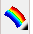
\includegraphics{contourFillIcon.png} and select: "WATER PRESSURE", then "DISPLACEMENT -> X-DISPLACEMENT" and lastly,"DISPLACEMENT -> y-DISPLACEMENT". Check if the contours are the same as shown in Figure \ref{fig:tut1_p1_results}
	
	\begin{figure}[h!]		
		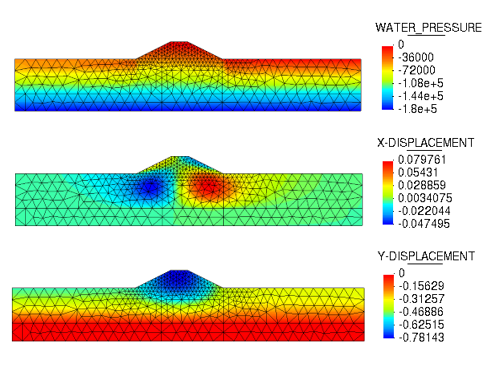
\includegraphics[width=\textwidth]{resultsTutorial1Part1.png}
		\caption{Contour results tutorial 1 part 1, top to bottom: water pressure, x-displacement, y-displacement}
		\label{fig:tut1_p1_results}
	\end{figure}

	\item Go back to the pre-process window. If the results are equal go on to the next part of the tutorial, if not, check if all input is correctly filled in.
	
\end{enumerate}

\section{Staged construction}
\begin{enumerate}[resume]
	\item While Kratos GeoMechanics can handle staged calculation, the GiD problemtype can not. In order to perform a staged calculation, some additional actions have to be performed within and outside the Gid pre-processor. The following stages will be added:
	\begin{itemize}
		\item Initial stage
		\item Addition of dike load
		\item Addition of daily water level
		\item High water level
	\end{itemize}
	
	\item Stage 1:
	\begin{enumerate}
		\item Save the existing file as \verb|"tutorial_1_stage_1"|
		
		\item Go to \textit{GeoMechanicsApplication -> Dirichlet Constraints -> Excavation}. Select the option \textit{Deactivate soil}. Name the condition \verb|dike_excavation| and assign the condition to the surfaces 7 and 8. 
		
		\item Go to \textit{GeoMechanicsApplication -> Problem data}. On the Problem data tab, set start and end time from 0.0 to 1.0.
		
		\item On the Solver Settings tab, set Solution type to K0- procedure. And set the Displacement Relative Tolerance on 1e-3.
		
		\item Re-mesh. 
		
		\item Click on Calculate and then cancel process. Note that clicking on Calculate is necessary to generate the input files. Results of the in between stages are not relevant, therefore it is not required to wait until the calculation is finished.
		\item Save the project again
	\end{enumerate}

	\item Stage 2
		\begin{enumerate}
		\item Save the existing file as \verb|"tutorial_1_stage_2"|
		
		\item Go to \textit{GeoMechanicsApplication -> Dirichlet Constraints -> Excavation}. Deselect the option \textit{Deactivate soil} of the \verb|dike_excavation| condition.
		
		\item Go to \textit{GeoMechanicsApplication -> Problem data}. On the Problem data tab, set start and end time from 1.0 to 2.0.
		
		\item On the Solver Settings tab, set Solution type to Quasi-Static.
		
		\item Re-mesh. 
		
		\item Click on Calculate and then cancel process.
		\item Save the project again
	\end{enumerate}

	\item Stage 3
	\begin{enumerate}
		\item Save the existing file as \verb|"tutorial_1_stage_3"|
		
		\item Go to \textit{GeoMechanicsApplication -> Problem data}. On the Problem data tab, set start and end time from 2.0 to 3.0.
		
		\item Click on Calculate and then cancel process.
		
		\item Save the project again
	\end{enumerate}
	
	\item Stage 4
	\begin{enumerate}
		\item Save the existing file as \verb|"tutorial_1_stage_4"|
		
		\item Go to \textit{GeoMechanicsApplication -> Problem data}. On the Problem data tab, set start and end time from 3.0 to 4.0.
		
		\item  Go to \textit{GeoMechanicsApplication -> Dirichlet Constraints -> Fluid Pressure}, set Y 2 of the dike \verb|dike_level| condition on -19. 
		
		\item Click on Calculate and then cancel process.
		
		\item Save the project again
	\end{enumerate}
		
\end{enumerate}

\section{Calculate staged construction}
A staged calculation cannot be calculated via GiD. This has to be done via the command prompt or python.
\begin{enumerate}[resume]
	\item Take the template file "MainKratos$\_$multiple$\_$stages$\_$template.py" from ./KratosGeoMechanics/applications/GeoMechanicsApplication. And copy it to the main KratosGeoMechanics directory. Rename the file to "MainKratos.py"
	
	\item right click on "MainKratos.py" and select "edit". 
	\item Edit the project$\_$paths variable such that it refers to the correct *.gid files. Note that the file paths should stay within the quotation marks.
	
	\item In windows explorer, go to the KratosGeoMechanics directory. In the adress-bar, type in: "cmd" and press "enter", such that command prompt is opened while already referring to the correct directory. In the command prompt, type in: "runkratos MainKratos.py". Now the calculation should start running with as many stages as preferred. 
	
\end{enumerate}

\section{Post-process part 2}
when all the stages are calculated, all the stages can be viewed separately in post process.

\begin{enumerate}[resume]
	\item In GiD go to post-processing. 
	\item Select "Open PostProcess" and go to the directory of your preferred stage. Click on the *.bin file to open the postprocess file. 
	\item Note that "DISPLACEMENT" shows the displacement of the current stage. "TOTAL$\_$DISPLACEMENT" shows the total displacement over the previously calculated stages. 
	
\end{enumerate}


	
